\documentclass[11pt,a4paper]{article}
\usepackage{theme/lmuthesis}

\usepackage[T1]{fontenc}
\usepackage[english]{babel}
\usepackage{unicode-math}
\usepackage{amsmath, amsfonts}
\usepackage{wasysym}
\usepackage{amsthm, thmtools}
\declaretheorem[numberwithin=section]{lemma, proposition, theorem, corollary}
\declaretheorem[numberwithin=section, style=plain]{example}
\declaretheorem[style=definition, numberwithin=section]{definition}
\declaretheorem[style=remark, numberwithin=section]{remark}

\usepackage{epstopdf}
\usepackage{tikz}
\usetikzlibrary{positioning, chains, shapes.geometric, fit, shapes, arrows.meta, calc, backgrounds, intersections, patterns, shapes.misc, fadings, through,decorations.pathreplacing}

\usepackage{pgfplots}

\usepackage{physics}
\usepackage{algorithm}
\usepackage{algpseudocode}

% this for draft water mark
\setboolean{release}{true}
\IfFileExists{condition}{\input{condition}}{}
\ifthenelse{\boolean{release}}{
}{
    \usepackage{draftwatermark}
    \SetWatermarkText{DRAFT}
    \SetWatermarkScale{1}
}

% meta informations
\department{Institut für TODO}
\lfe{Lehr- und Forschungseinheit TODO}
\professor{Prof.\ Dr.\ PROFESSORS NAME}
\type{Bachelor's Thesis}
\title{THESIS TITLE}
\author{Valentin Herrmann}
\email{EMAIL}
\bearbeitungszeitraum{START bis END}
\supervisor{SUPERVISOR}
\taskdescription{
    \begin{description}
        \item[THESIS TITLE]
        \item[Problem Statement] TO BE ADDED
        \item[Scope of the Thesis] TO BE ADDED
        \item[Tasks] TO BE ADDED
        \item[Requirements] TO BE ADDED
        \item[Keywords] TO BE ADDED
    \end{description}
}
\acknoledgement{
    I would like to appreciate ...
}
\abstract{
    This thesis proposes ...
}

\newcommand{\dtlifsnn}{d.t. LIF-SNN }
\newcommand{\Dtlifsnn}{d.t. LIF-SNN }
\newcommand{\rdtlifsnn}{r. d.t. LIF-SNN }
\newcommand{\Rdtlifsnn}{R. d.t. LIF-SNN }
\newcommand{\proofofref}[1]{Proof of~\autoref{#1}.}

\begin{document}

\makecover
%\maketaskdescription
%\makededication
\makeabstract
\maketoc
% optional:
% \listoffigures
% \listoftables
\cleardoublepage

\section{Introduction}
\label{ch:intro}

While the hype on AI is still ongoing there are still people wondering if current AI models are fundamentally able of reasoning. Many other possible models could be better fitted to the task of reasoning. Among others Spiking neural networks present a model closer to the workings of the brain. In fact, they have been called the 3rd generation of AI models, after the 2nd generation that currently drives most successful models.

While the idea behind SNNs is quite old, they have not been as much researched, since it is much more inefficient and harder to train them. Therefore there still remain a lot of open questions about them.
In this paper we shall extend on the work done in~\cite{nguyen2025timespikeunderstandingrepresentational}. We will add a decaying factor to the input of the neurons and allow recursive connections between neurons in a layer.

We will roughly follow the structure of~\cite{nguyen2025timespikeunderstandingrepresentational}. In the second chapter we will formally introduce discrete time leaky-integrate-and-fire SNN, d.t. LIF-SNNs. In section 3 we will give theorems about approximation of continuous functions on compact domains by d.t. LIF-SNNs.
The main part will be the following section in which we will see that the number of distinct values a d.t. LIF-SNN can take on only depends on the first hidden layer and grows in particular only quadratically in time. We will further support our findings with experimental data in the last section.
% approximation of differentiable ones?
 \cleardoublepage
\section{Definitions}
\label{ch:defs}

%TODO: Bild
Our type of SNN should be thought of as a composition of an initial input layer, a number of hidden spiking layers with internal state and an affine-linear layer mapping spikes activations over time, so called spike trains, to the value of the output layer.
The following definitions deviate slightly from~\cite{nguyen2025timespikeunderstandingrepresentational}, since we already bake in some of the assumptions (direct encoding and membrane-potential outputs) the paper makes at a later point.
We shall first define the membrane potential \(u^l(t)\) and the spike activations \(s^l(t)\) of the hidden layers:

%TODO: herleitung
\begin{definition}
  The \textbf{input vector} \(i^l(t)∈\{0,1\}^{n_l}\), the \textbf{spike vector} \(s^l(t)∈\{0,1\}^{n_l}\) and the \textbf{membrane potential vector} \(u^l(t)\) of a hidden layer \(l∈[L]\) are recursively defined as
  \begin{align}
    i^l(t) & = α^li^l(t-1)+W^ls^{l-1}(t)+V^ls^l(t-1) \\
    p^l(t) & = β^lu^l(t-1)+i^l(t)+b^l \\
    s^l(t) & = H(p^l(t)-ϑ1_{n_l}) \\
    u^l(t) & = p^l(t)-ϑs^l(t)
  \end{align}
  with \(s^l(0)=0\) and given
  \begin{enumerate}
    \item[•] \textbf{first layer spike activations}: \((s^0(t))_{t∈[T]}∈\{0,1\}^{n_0×T}\)
    \item[•] \textbf{initial membrane potential}: \(u^l(0)∈ℝ^{n_l}\)
    \item[•] \textbf{initial input}: \(i^l(0)∈ℝ^{n_l}\)
    \item[•] \textbf{weight matrices}: \(W^l∈ℝ^{n_l×n_{l-1}}\)
    \item[•] \textbf{bias vectors}: \(b^l∈ℝ^{n_l}\)
    \item[•] \textbf{leaky terms}: \(α^l,β^l∈[0,1]\)
    \item[•] \textbf{threshold}: \(ϑ^l∈(0,∞)\)
  \end{enumerate}
  where \(H≔𝟙_{[0,∞)}\) is a step function and \(T∈ℕ\) is the number of simulated time steps.
\end{definition}

In the definition of \(s^l(t)\) we first check whether the additional activation by spikes \(W^ls^{l-1}(t)\) of the previous layers and the bias \(b^l\) plus the decayed previous activation \(β^lu^l(t-1)\) passes over a certain threshold \(ϑ^l1_{n_l}\). If that is not the case we use the just computed value for \(u^l(t)\). If the neuron activates, we remove a threshold worth of value. Of course, we do this for the neurons of the whole layer in parallel.

We further define d.t. LIF-SNN and the function the network realizes:

\begin{definition}
  A \textbf{discrete-time LIF-SNN} of \textbf{depth} \(L\) with \textbf{layer-widths} \((n_0,…,n_{L+1})\) is given by
  \[ Φ≔((W^l,b^l,u^l(0),i^l(0),α^l,β^l,ϑ^l)_{l∈[L]},T,((a_t)_{t∈[T]},c,V) \]
  where \((a_t)_{t∈[T]}∈ℝ^T\), \(c∈ℝ^{n_{L+1}}\) and \(V∈ℝ^{n_{L+1}×n_L}\) are the parameters of the output layer.
\end{definition}

\begin{definition}
  A discrete-time LIF-SNN \(ϕ\) \textbf{realizes} the function \(R(Φ):ℝ^{n_0}→ℝ^{n_{L+1}}\):
  \[ R(Φ)(x)=D((s^L(t))_{t∈[T]})\quad \text{with }s^0(t)≔x\]
  where the last layer \(D\) is defined by \( D((s(t))_{t∈[T]})=\sum^T_{t=1}a_t(Vs(t)+c)\).
\end{definition}

Let us now take a look at some simple examples:

\begin{example}
  Let \(T,L∈ℕ\). Then there exists a d.t. LIF-SNN with \(∀_{t∈[T]}s^L(t)=s^0(t)\) for any \(s^0∈\{0,1\}^{n_0×T}\).

  We can proof this by using constant width \(n_l=n\), weights \(W^l=I_n\), biases \(b^l=0\), initial membrane potential \(u^l(0)=0\), leaky term \(β^l=0\) and threshold \(ϑ^l=1\) for all \(l∈[L]\).

  We then get by definition:
  \begin{alignat*}{3}
    s^l(t) & = H(& s^{l-1}(t)-1_{n_l})  &= \ s^{l-1}(t) \\
    u^l(t) & = & s^{l-1}(t)-s^l(t)     &= 0
  \end{alignat*}
\end{example}

\begin{example}\label{ex:2}
  Let \(T,L∈ℕ\). Then there exists a d.t. LIF-SNN with \(∀_{t∈T}s^L(t)=\max_{t'∈[t-1]}(s^0(t'))\) for any \(s^0∈\{0,1\}^{n_0×T}\): In this network an output neuron switches on when the corresponding input neurons fires and does not switch off later.

  We can proof this by using constant width \(n_l=n\), weights \(W^l=T·I_n\), biases \(b^l=0\), initial membrane potential \(u^l(0)=0\), leaky term \(β^l=1\) and threshold \(ϑ^l=1\) for all \(l∈[L]\).

  We then get by definition:
  \begin{alignat*}{2}
    s^l(t) & = H(&u^l(t-1)+T·s^{l-1}(t)-1_{n_l}) \\
    u^l(t) & = &u^l(t-1)+T·s^{l-1}(t)-s^l(t)
  \end{alignat*}
  By adding over all timesteps we obtain
  \begin{alignat*}{1}
    s^l(t) & = H(T\sum_{i=1}^ts^{l-1}(i)-(\sum_{t=i}^{t-1}s^l(i))+1_{n_l}) ) \\
    u^l(t) & = \sum_{i=1}^t(T·s^{l-1}(i)-s^l(i))
  \end{alignat*}
  Since \(\sum_{i=1}^{t-1}s^l(i)+1_{n_l}≤T\), once there is any \(t_0∈[T]\) with \(s^{l-1}_i(t_0)=1\) for an \(i\), we get \(∀_{t≥t_0}s^l_i(t)=1\).
  By induction over the layers we clearly get the required property.
\end{example}

\cleardoublepage
 \cleardoublepage
\section{Structure of computations in \rdtlifsnn s}
\label{ch:struct}

This section concern itself with the approximation of continuous functions by d.t. LIF-SNN.

In~\cite{nguyen2025timespikeunderstandingrepresentational} the following theorem was proved:
\begin{theorem}\label{thm:approx-snn-constant}
  Let \(f\) be a continuous function on a compact set \(Ω⊂ℝ^{n_0}\). For all \(ε>0\), there exists a d.t. LIF-SNN \(Φ\) with direct encoding, membrane potential output, \(L=2\) and \(T=1\) such that
  \[ \norm{(R(Φ)-f)|_{Ω}}_{∞}≤ε\]
  Moreover, if \(f\) is \(Γ\)-Lipschitz, then \(Φ\) can be chosen with width parameter \(n=(n_1,n_2)\) given by
  \begin{align*}
   n_1 &=\left(\max\left\{\left\lceil \frac{\operatorname{diam}_∞(Ω)}{ε}Γ \right\rceil,1\right\}+1\right)n_0  \\
   n_2 &=\max\left\{\left\lceil \frac{\operatorname{diam}_∞(Ω)}{ε}Γ \right\rceil^{n_0},1\right\}
  \end{align*}
  where \(\operatorname{diam}_∞(Ω)=\sup_{x,y∈Ω}\norm{x-y}_∞\).
\end{theorem}

\begin{proof}
  See~\cite{nguyen2025timespikeunderstandingrepresentational}.
\end{proof}

\begin{figure}[h!]
  \begin{subfigure}[t]{0.45\textwidth}
    \centering
    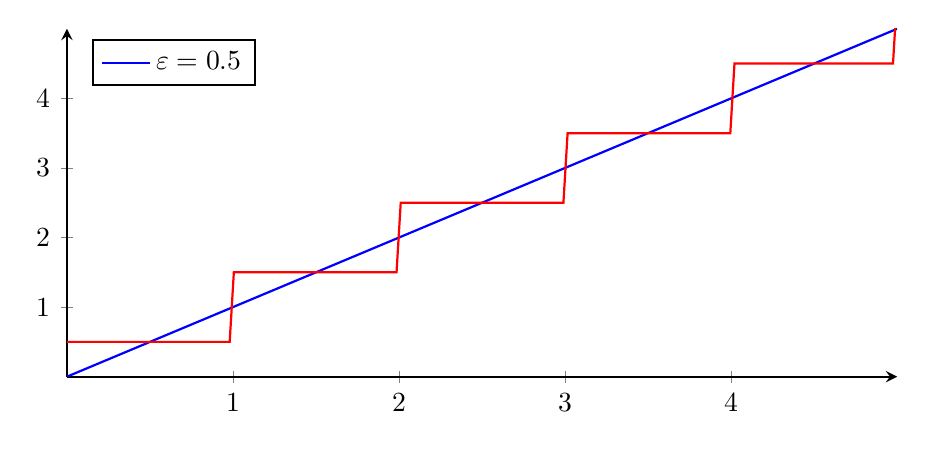
\begin{tikzpicture}
      \begin{axis}[
        axis lines=middle,
        xmin=0, xmax=5,
        ymin=0, ymax=5,
        xtick={0, 1, 2, 3, 4},
        ytick={0, 1, 2, 3, 4},
        domain=0:5,
        samples=200,
        thick,
        legend pos=north west,
        width=\textwidth,
        height=6cm
        ]
        \addplot[blue]{x};
        \addplot[red]{floor(x)+0.5};
        \addlegendentry{$ε=0.5$}
      \end{axis}
    \end{tikzpicture}
    \caption{A \dtlifsnn approximating the identity}
    \label{id:sin-approx-by-dtlifsnn}
  \end{subfigure}
  \hfill
  \begin{subfigure}[t]{0.55\textwidth}
    \centering
    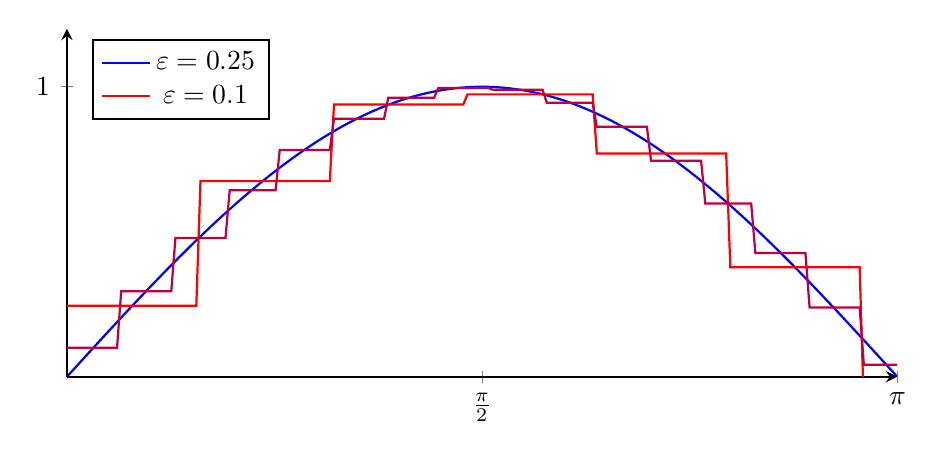
\begin{tikzpicture}
      \begin{axis}[
        axis lines=middle,
        xmin=0, xmax=pi,
        ymin=0, ymax=1.2,
        xtick={0, pi/2, pi},
        xticklabels={$0$, $\frac{\pi}{2}$, $\pi$},
        ytick={0, 1},
        domain=0:pi,
        samples=200,
        thick,
        legend pos=north west,
        width=\textwidth,
        height=6cm
        ]
        \addplot[blue]{sin(deg(x))};
        \addplot[red]{(-cos(deg(floor(x*2+1)/2))+cos(deg(floor(x*2)/2)))*2};
        \addlegendentry{$ε=0.25$} % ε≈0.5*(1/2) (since sin(x)≈x for x≪1)
        \addplot[purple]{(-cos(deg(floor(x*5+1)/5))+cos(deg(floor(x*5)/5)))*5};
        \addlegendentry{$ε=0.1$} % ε≈0.5*(1/5) (since sin(x)≈x for x≪1)
      \end{axis}
    \end{tikzpicture}
    \caption{A \dtlifsnn approximating a sinus wave}
    \label{fig:sin-approx-by-dtlifsnn}
  \end{subfigure}
\end{figure}

The proof of~\cref{thm:approx-snn-constant} works by first showing that a continuous function can be arbitrarily approximated by step functions, in particular by step functions constant on hypercubes in \(Ω\).
Then the \dtlifsnn is constructed by using the first layer to cut the input space by hyperplanes along the cubes and using the second layer to represent the hypercubes.

While quite simple, this construction does not use the unique feature of (r.) \dtlifsnn, the ability of neurons to accumulate state over time. It therefore needs quite a lot more neurons than actually needed for many functions with (almost) linear segments, e.g. a sinus wave, see also~\cref{fig:sin-approx-by-dtlifsnn}.

We will now show a more efficient construction for \rdtlifsnn that uses the fact that \rdtlifsnn can quite efficiently approximate linear segments. The general intuition behind is to use piece-wise linear functions to approximate continuously differentiable functions and then approximate those piece-wise linear functions by \rdtlifsnn. In the end, we will see that we can in fact approximate any continuous function like this, by using mollification to extract an continuously differentiable approximation of the function.

% TODO: motivation (previous theorem + previous lower bound example), insatisfactory since d.t. SNN. have somewhat linear structure

% TODO: extend to arbitrarily continuous functions by choosing an continuously diff. function close to it
% TODO: extend to continuously differentiable functions apart from lebesgue-zero sets (where they are still continuous?)
% TODO: differentiable, but defined on compact subset of euclidean space???
%
% TODO: use generalized inverse of the modulus of continuity

%TODO: demand differentiability only for Ω°
We will now provide an alternative version of this theorem which uses an increased latency to reduce the number of neurons:
\begin{theorem}\label{thm:approx-snn}
  Let \(f∈𝒞^1(U,ℝ^m)\), with \(∅≠U⊂ℝ^n\) open, be a continuously differentiable function. Let further \(Ω⊂U\) be a compact set. For all \(ε,μ,ν>0\), \(ε=μ+ν\), there exists a \rdtlifsnn \(Φ\) with \(L=3\) and
  \begin{align*}
   T   &= (K(μ)+1)T_r(ν)+1 \\
   n_1 &= n+1 \\
   n_2 &= K^n(μ)·(n+1)+3
  \end{align*}
  such that
  \[ \norm{(R(Φ)-f)|_{Ω}}_{∞,2}≤ε.\]
  Here \(T_r≔T_r(ν)≔\frac{\operatorname{diam}(Ω)}{K}\frac{\norm{f'}_{∞,2}}{2ν}\).
  The definition of \(K(μ)\) is given in~\cref{lem:approx-by-lin}.
\end{theorem}

\begin{lemma}\label{lem:smallest-cube}
  Let \(Ω⊂ℝ^n\) be compact. Then there exists a half-open cube \(C\) with width \(\operatorname{diam}_∞(Ω)\) such that \(Ω⊂\overline{C}\).
\end{lemma}

%TODO: we later use ⟦y,z⦆ instead of ⟦a,b⦆; unify notation
\begin{proof}[\proofofref{lem:smallest-cube}.]
  We can first define \(x≔(\min_{x∈Ω} x_i)_i\) since \(Ω\) is compact We further have \(y≔x+\operatorname{diam}_∞(Ω)·𝟙_n\). We now have \(C≔⟦x,y⦆\). Suppose now a point \(z∈Ω∖\overline{C}\) exists. By definition of \(x\), we have \(x≤z\). By definition of \(C\) we further get \(z\nleq y\), and therefore \(∃_iy_i<z_i\) by definition of \(C\). But this means \(\norm{x-z}_∞>\operatorname{diam}_∞(Ω)\).
\end{proof}

\begin{comment}
\begin{lemma}\label{lem:uniform-cont-≤}
  Let \(M\) be a normed vector space and \(N\) be a metric space. Let \(f:M→N\) be uniformly continuous with modulus \(δ\). We then have for every \(ε>0\):
  \[ ∀_{x,y∈M}(\norm{x-y}_M≤δ(ε)⇒d_N(x,y)≤ε). \]
\end{lemma}

\begin{proof}
  Let \(ε>0\) with modulus \(δ(ε)\), as well as \(x∈M\) be given. Since \(f\) is uniformly continuous with modulus \(δ(ε)\), we have \(f(B_{δ}(x))⊂B_{ε}(f(x))\). Since \(f\) is in particular continuous, we get
  \[ f(\overline{B}_{δ}(x))=f(\overline{B_{δ}(x)})⊂\overline{f(B_{δ}(x))}⊂\overline{B}_{ε}(f(x)) \]
  We need to use the fact that \(M\) is a normed vector space in the first equality to get \(\overline{B}_{δ}(x)=\overline{B_{δ}(x)}\).
\end{proof}
\end{comment}

\begin{lemma}\label{lem:inverse-cont-mod}
  Let \(ω:[0,∞]→[0,∞]\) be a modulus of uniform continuity of a uniformly continuous function \(f:M→N\), where \(M,N\) are metric spaces. We then define the generalized inverse of \(ω:[0,∞]→[0,∞]\) by \(ω^{†}(s)≔\inf\{t∈[0,∞]\mid ω(t)>s\}\).

  We have the following properties
  \begin{enumerate}
  \item \(∀_{x,y∈M,s∈[0,∞]}d_M(x,y)≤ω^{†}(s)⇒d_N(f(x),f(y))≤s\).
  \item \(∀_{s∈[0,∞]}s=0⇔w^{†}(s)=0\).
  \end{enumerate}
\end{lemma}

\begin{proof}\phantom{}

  \begin{enumerate}
  \item Let \(x,y∈M\) and \(s∈[0,∞]\) be given such that \(d_M(x,y)≤ω^{†}(s)\). By definition of \(ω^{†}\), this means \(ω(d_M(x,y))≤s\). Since \(ω\) is a modulus of uniform continuity of \(f\), we have \(d_N(f(x),f(y))≤ω(d_M(x,y))\) and therefore overall \(d_N(f(x),f(y))≤s\).
  \item Since \(ω\) is a modulus of uniform continuity, it is by definition continuous at \(0\). Let us choose an arbitrary sequence \((t_n)_{n∈ℕ}\) with \(t_n→0\). Then \(ω(t_n)→0\) and therefore \(ω^{†}(0)≤\inf_{n∈ℕ}t_n=0\).

  Is on the other hand \(ω^{†}(s)=0\), then there is a sequence \((t_n)_{n∈ℕ}\) with \(t_n→0\) and therefore \(ω(t_n)→0\). By definition of \(ω^{†}(s)\), we have \(ω(t_n)>s\), so we get \(s=0\).
  \end{enumerate}
\end{proof}

% TODO: differentiable, but defined on compact subset of euclidean space???
% TODO: quote formulation?
% TODO: instead of fixing \(ε^{t}\), get supremum of
% TODO: why K≠0?
% TODO: only demand differentiability on C°

\begin{lemma}\label{lem:approx-by-lin}
  Let \(f∈𝒞^1(U,ℝ^m)\), with \(∅≠U⊂ℝ^n\) open, be a continuously differentiable function. Let further \(Ω⊂U\) be a compact set, such that there is a half-open cube \(C\) with \(Ω⊂\overline{C}⊂U\).

  For every \(μ>0\) we can compose \(C\) into
  \[ K^n≔K(μ)^n≔\min_{\substack{ξ,θ>0\\ξθ=μ}}\left\{\left\lceil \frac{\operatorname{diam}_∞(Ω)}{\frac{2}{\sqrt{n}}\min(ω^{†}(ξ) ,θ)} \right\rceil\right\}^n \]
  half-open subcubes \((C_i)_{i=1..K^n}\) such that affine linear functions \(g_i:C_i→ℝ^m\) exist with \(\norm{f-g}_{∞,2}<μ\), where \(g\) is the continuous extension of \((\sum_{i=1}^mg_i𝟙_{C_i})|_C\) on \(\overline{C}\).
  Here \(ω^{†}\) is the generalized inverse of a modulus of uniform continuity (with regard to \(\norm{·}_2\)) of the total derivative \(dF|_{\overline{C}}\). Since \(ξ>0\), we also have \(ω^{†}(ξ)>0\) by~\cref{lem:inverse-cont-mod}.
\end{lemma}

\begin{remark}{}\\
\begin{enumerate}
\item If \(f∈𝒞^1(U,ℝ^m)\) is given with \(∅≠U⊂ℝ^n\) and a compact \(Ω⊂ℝ^n\), but with no half-open cube \(C\) such that \(Ω⊂\overline{C}⊂U\), we can extend \(f|_{Ω}\) to a function \(f'∈𝒞^1(ℝ^n,ℝ^m)\): There is a partition of one \(φ_1,φ_2∈𝒞^{∞}(ℝ^n)\) subordinate to \(U\) and \(ℝ^n∖Ω\). We get \(φ_1|_{Ω}=1\) and therefore \((φ_1f)|_{Ω}=f|_{Ω}\). \(f'≔φ_1f\) is further clearly \(𝒞^1(U,ℝ^m)\).
% \item We would like to only demand differentiability on \(Ω°\), … %TODO
\end{enumerate}

%TODO ↓
  % We would like to only demand differentiability on \(Ω°\), but the theorem would not be true anymore. Imagine the function \(f(x)=χ_{[0,1]}\) with \(Ω=[0,1]∪[2,3]\). Clearly, \(f|_{[0,1]∪[2,3]}\) is continuous and \(f|_{(0,1)∪(2,3)}∈𝒞^1(ℝ)\). But on the other hand a half-open cube around \(Ω\) at least needs to include \((1,2)\) and would need to have
\end{remark}

% TODO: remark about why we are using 2-norm

% TODO: fix issue with C_i s not completely fitting in open \sqrt{2}δ(μ) balls due to closed part of C_i
% TODO: F might not be defined at c_i, since \(Ω≠\overline{C}\)
\begin{proof}[\proofofref{lem:approx-by-lin}.]
  By~\cref{lem:smallest-cube} we have a half-open cube \(C\) with width \(\operatorname{diam}_∞(Ω)\) and \(Ω⊂\overline{C}\). We can assume w.l.o.g. we can assume \(\overline{C}⊂U\), since we can extend \(f\) to a function \(f'∈𝒞^1(ℝ^n,ℝ^m)\):

  Let further \(μ>0\) be given. Since \(Ω\) is compact and \(f∈𝒞^1(Ω,ℝ^m)\), \(dF\) is uniformly continuous on \(Ω\). Let \(ω\) be a modulus of uniform continuity of \(dF\mid_{Ω}\).
  We will now partition \(C\) in
  \[K^n≔\min_{\substack{ξ,θ>0\\ξθ=μ}}\left\{\left\lceil \frac{\operatorname{diam}_∞(Ω)}{\frac{2}{\sqrt{n}}\min(ω^{†}(ξ) ,θ)} \right\rceil\right\}^n\]
  smaller half-open cubes. There are \(ξ,θ\) such that the minimum in the definition of \(K^n\) is obtained, since we take it over the set of natural numbers. \(K\) is further well-defined, since \(∀_{s>0}ω^{†}(s)>0\),
  The subcubes have width \(w≔\frac{\operatorname{diam}_∞(Ω)}{K}≤\frac{2}{\sqrt{n}}\min(ω^{†}(ξ),θ)\). % TODO: should be < instead of ≤ in def of w???

  %TODO: why do we not have to proof <μ on the boundary of C, on the extension

  Let us further define \(g_i:C_i→ℝ^m\) by \(g_i(x)≔f(c_i)+df_{c_i}(x-c_i)\) where \(c_i\) is the center of \(C_i\), so in particular
  \begin{equation}\label{eq:4}
  \norm{x-c_i}_2=\sqrt{\sum_{j=1}^n\norm{(x-c_i)_je_j}_2^2}≤\frac{w}{2}\sqrt{n}≤\min(ω^{†}(ξ),θ).
  \end{equation}

  It suffices now to show \(\norm{f|_{C_i}-g_i}_∞<μ\). Let \(x∈C_i\) and \(h(t)≔f(t(x-c_i)+c_i)\) with
  \[h'(t)=(df_{(x-c_i)t+c_i}∘d(t↦t(x-c_i)+c_i)_t)(1)=df_{(x-c_i)t+c_i}(x-c_i).\]
  We obtain by the Fundamental theorem of calculus:
  \begin{align*}
  \norm{f(x)-f(c_i)-df_{c_i}(x-c_i)}_2 &= \norm{h(1)-h(0)-df_{c_i}(x-c_i)}_2 \\
                                    &= \norm{\int_0^1df_{(x-c_i)t+c_i}(x-c_i)dt-df_{c_i}(x-c_i)}_2
  \end{align*}
  Due to the generalized Minkowski-Inequality we can move the norm inside the integral:
  %TODO: ref for gen. Minkowski-Ineq?
  \begin{align*}
   \norm{\int_0^1df_{(x-c_i)t+c_i}(x-c_i)dt-df_{c_i}(x-c_i)}_2 &≤ \int_0^1\norm{df_{(x-c_i)t+c_i}(x-c_i)-df_{c_i}(x-c_i)}_2dt \\
                                    &= \int_0^1\norm{(df_{(x-c_i)t+c_i}-df_{c_i})(x-c_i)}_2dt \\
                                    &≤ \int_0^1\norm{df_{(x-c_i)t+c_i}-df_{c_i}}\norm{x-c_i}_2dt \\
                                    &≤ \int_0^1ξ\norm{x-c_i}_2dt \\ % w≤2\sqrt{n}^{-1}ω^{†}(ξ) %TODO: should be <???
                                    &= ξ\norm{x-c_i}_2 \\
                                    &≤ ξθ \\
                                    &= μ
  \end{align*}
  In the fourth step we use \(\norm{df_{(x-c_i)t+c_i}-df_{c_i}}≤ξ\), which holds due to \(∀_{t∈[0,1]}(x-c_i)t+c_i∈C_i\), \eqref{eq:4} and \cref{lem:inverse-cont-mod}.
\end{proof}
%TODO: change notation of c_i to sth clearly not meant component

\begin{proof}[\proofofref{thm:approx-snn}.]
  Let a continuously differentiable function \(f∈𝒞^1(Ω,ℝ^m)\) on a compact set \(Ω⊂ℝ^n\) be given. Let there further be \(ε,μ,ν>0\) with \(ε=μ+ν\).
  %TODO: clarify notation ⟦y,z⦆ (line or proper subspace)
  By~\cref{lem:approx-by-lin} we have a half-open cube \(C=⟦x^C,y^C⦆\) with \(Ω⊂C\) with composition \(K^n\) half-open subcubes \((C_i)_{i=1..K^n}\) and linear functions \(g_i:C_i→ℝ^m\), such that \(\norm{f-g|_Ω}_∞<μ\) for a \(g≔\sum_{i=1}^mg_i𝟙_{C_i}\).

  We will now define a \rdtlifsnn \(Φ\) with direct input encoding and membrane-potential outputs such that \(\norm{R(Φ)|_Ω-g}_∞<ν\).

  Before anything else we shall set the following basic parameters \(i^{[l]}(0)=0\), \(α^{[l]}=0\) and \(β^{[l]}=ϑ^{[l]}=1\) for all layers.

  % TODO: graphic

  The intuitive idea for the construction of the network is the following: In the first layer we have \(n\) neurons which capture the position of the input vector regarding \(C\) in their respective dimension and one last neuron that acts as an “alarm clock” that shuts down the other neurons of the layer after the first \(KT_r\) time steps.

  The general idea of the second layer is that it just listens for the first \(KT_r\) time steps to the first layer and then in time-step \(KT_r+1\) it is decided which region \(C_i\) the input is located in. The last \(T_r\) time-steps are used to encode the location of \(x\) inside of \(C_i\).

  For each region \(C_i\) we have \(n+1\)-neurons. Each of the first \(n\) neurons encodes a commponent of the linear part of \(g_i\). They are also used to inform the \(n+1\)-th neuron of the group if the \(x\) has at least as big as the base point of \(C_i\). The \(n+1\)-th deactivates all other neurons of regions with smaller base point and encodes the constant part of \(g_i\). The last \(3\) neurons act as “clock neurons” enabling and disabling the other ones.

  % In the second layer we have \(m+1\)-neurons for each affine linear region \(C_i\). Each of the first \(m\) neurons encodes the linear part of a component of the output vector. The last, additional neuron acts as an activator to the specific region by recursively enabling the other neurons of this region and disabling all regions with smaller base point (that would otherwise be enabled).

  \begin{figure}[h]
    \centering
    \tikzstyle{descript} = [text = black,align=center, minimum height=1.8cm, align=center, outer sep=0pt,font = \footnotesize]
\tikzstyle{activity} =[align=center,outer sep=1pt]
\definecolor{ColorOne}{named}{MidnightBlue}
\definecolor{ColorTwo}{named}{Dandelion}
\definecolor{ColorThree}{named}{Plum}
\begin{tikzpicture}[very thick, black]
  \small
  %% Coordinates
  \coordinate (O) at (0,0); % Origin
  \coordinate (P1) at (4,0);
  \coordinate (P2) at (8,0);
  \coordinate (F) at (13,0); %End
  \coordinate (E1) at (5,0); %Event
  %% Filled regions
  \fill[color=ColorOne!20] rectangle (O) -- (P1) -- ($(P1)+(0,1)$) -- ($(O)+(0,1)$); % Studies
  \path [pattern color=ColorOne, pattern=north east lines, line width = 1pt, very thick] rectangle ($(O)+(0.5,0)$) -- ($(O)+(2,0)$) -- ($(O)+(2,1)$) -- ($(O)+(0.5,1)$); % Something else
  \fill[color=ColorTwo!20] rectangle (P1) -- (P2) -- ($(P2)+(0,1)$) -- ($(P1)+(0,1)$); % Work
  %% Text inside filled regions
  \draw ($(P1)+(-2.5,0.5)$) node[activity,ColorOne] {Studies};
  \draw ($(P2)+(-2,0.5)$) node[activity,ColorTwo] {Work};
  % \draw ($(P3)+(-2,0.5)$)  node[activity, ColorThree] {Current activity};

  %% Events
  \draw[<-,thick,color=black] ($(E1)+(0,0.1)$) -- ($(E1)+(0,1.5)$) node [above=0pt,align=center,black] {Unexpected\\event};
  %% Arrow
  \draw[->] (O) -- (F);
  %% Ticks
  \foreach \x in {0,2,...,12}
  \draw(\x cm,3pt) -- (\x cm,-3pt);
  %% Labels
  \foreach \i \j in {0/0,2/T_r(θ),4/2T_r(θ),10/K(ξ)T_r(θ),12/T}{
    \draw (\i,0) node[below=3pt] {$\j$} ;
  }
\end{tikzpicture}

% adapted from https://www.overleaf.com/project/68b326ec3dceb466ee45cc28

    \caption{Timeline of first-layer neuron}
  \end{figure}

  \begin{enumerate}
  \item First layer:
  We define the \(i\)-th neuron of the \(n\) neurons of the first layer by parameters
  \[ w=\frac{1}{y^C_i-x^C_i}e_i, \quad b=-\frac{x^C_i}{y^C_i-x^C_i}, \quad v=-e_{n+1},\quad u_0=0, \quad i_0=0. \]
  The “clock neuron” of the first layer, with index \(c_1≔n+1\), is defined by:
  \begin{equation*}
    w=0, \quad b=\frac{1}{KT_r}, \quad v=e_{c_1}, \quad u_0=0, \quad i_0=0.
  \end{equation*}

  % TODO: check that proof works for x∈\(\overline{C}∖C\)

  % We further define the \(n+1\)-th neuron of the first layer by \(w=0\), \(b=\frac{1}{K-1}\), \(v=\)
  % By~\cref{lem:non-recursive-defs} we get

  % TODO: proof correct behaviour

  %TODO: add timeline
  \item Second layer:
  Let us now construct the second layer in the following way: For each of the \(K^n(μ)\) subcubes in \(C\) we define \(n+1\) neurons like so: Let \(C_j=⟦x^{C_j},y^{C_j}⦆\) be one such subcube with position \(q∈\{0,…,K(μ)-1\}^{n_1}\) in \(C\). We will write \(ι_j(i)≔j(n+1)+i\) to index the first \(n\) neurons in the layer and \(ω_j≔(j+1)(n+1)\) to index the last neuron of each group.

  The \(i\)-th neuron of the first \(n\) neurons, with index \(ι_j(i)\) in the second layer, has the parameters
  \begin{gather*}
    w=e_i, \quad b=0, \quad v=T(e_{c_2}-2e_{c_3}+e_{ω_j}-r(q)), \\
    u_0=-q_iT_r-T+1, \quad i_0=0.
  \end{gather*}
  where \(j(q)\) is the index of the subcube at position \(q\) and “the switch” is
  \[ r(q)≔e_{ω_j}-\sum_{\substack{q'∈\{0,…,K(μ)-1\}^{n_1} \\ q'<q}}e_{ω_j(q)}. \]
  The final neuron of the group, with index \(ω_j\) in its layer, has the parameters
  \begin{gather*}
    w=0, \quad b=0, \quad v=\frac{1}{n}\sum_{i=1}^ne_{ι_j(i)}+e_{ω_j}-e_{c_4}-r(q), \quad u_0=0, \quad i_0=0.
  \end{gather*}
  We also define the three “clock neurons”, with index \(c_2≔(j+1)K^n(μ)+1\), \(c_3≔(j+1)K^n(μ)+2\) and \(c_4≔(j+1)K^n(μ)+3\) with very parameters:
  %TODO: KT_r=1?
  \begin{equation*}
    w=0, \quad b=b_{c_i}, \quad v=-2e_{c_i}, \quad u_0=0, \quad i_0=0.
  \end{equation*}
  where \(b_{c_1}=\frac{1}{KT_r-1}\), \(b_{c_2}=\frac{1}{KT_r}\) and \(b_{c_3}=\frac{1}{KT_r}\).
  %TODO: use c_{-1}, c_0 and c_{1} and a (for alarm) for the first layer neuron.
  \item Output decoder:
  We further define the parameters of the output decoder by \(a_t=0\), for \(t≤KT_r+1\) and otherwise \(a_t=1\). We further set \(b^{[L+1]}=0\) and \((W^{[L+1]})_{l,ι_j(i)}=g(x^{C_j}+\frac{1}{T_r}e_i)-g(x^{C_j})\) for \(l∈[m]\), \(j∈K^n\) and \(i∈[n]\), as well as \((W^{[L+1]})_{l,ω_j}=g(x^{C_j})\) for \(l∈[m]\) and \(j∈K^n\).
  \end{enumerate}

  We will now proof that this construction indeed approximates \(g\) well enough. It will be helpful to consider the following, by choice of \(i^{[l]},α^{[l]},β^{[l]},ϑ^{[l]}\), simplified equations:
  \begin{align*}
    p^{[l]}(t) & = u^{[l]}(t-1)+W^{[l]}s^{[l-1]}(t)+V^{[l]}s^{[l]}(t-1)+b^{[l]} \\
    s^{[l]}(t) & = H(p^{[l]}(t)-1_{n_l}) \\
    u^{[l]}(t) & = p^{[l]}(t)-s^{[l]}(t)
  \end{align*}
  and in particular by~\cref{lem:non-recursive-defs}
  \begin{align*}
   i^{[l]}(t) &= W^{[l]}s^{[l-1]}(t)+V^{[l]}s^{[l]}(t-1)  \\
   p^{[l]}(t) &= u^{[l]}(0)+\sum_{k=1}^t\left(W^{[l]}s^{[l-1]}(k)+V^{[l]}s^{[l]}(k-1)+b^{[l]}\right)-\sum_{k=1}^{t-1}s^{[l]}(k).
  \end{align*}

  Let now \(s^{[0]}(t)=x∈C\). We will proof \(\norm{R(Φ)(x)-g(x)}_{∞,2}≤ν\) in steps, by first proofing some simple properties of the previously defined neurons:

  \begin{enumerate}
  \item Characterization of the “clock neuron” of the first layer:\\
  Let us first regard the neuron in the first layer: By choice of parameters we get:
  \begin{equation*}
   p^{[1]}_{c_1}(t) = \frac{t}{KT_r}+\sum_{k=1}^ts^{[1]}_{c_1}(k-1)-\sum_{k=1}^{t-1}s^{[1]}_{c_1}(k) = \frac{t}{KT_r}
  \end{equation*}
  So \(s^{[1]}_{c_1}(t)=1⇔t≥KT_r\).
  \item Characterization of \(i\)-th neuron of the first layer, “capturing” the \(i\)-th dimension:\\
  We have:
  \begin{align*}
   i^{[1]}_i(t)+b^{[1]}_i=\frac{x_i-x^C_i}{y^C_i-x^C_i}-s^{[1]}_{c_1}(t-1)
  \end{align*}
  So we can use~\cref{lem:sum-spikes-over-time} for \(x^C_i≤x_i<y_i^C\) and \(t≤KT_r\) to obtain
  \begin{equation*}
  \left\lfloor KT_r\frac{x_i-x^C_i}{y^C_i-x^C_i} \right\rfloor =\left\lfloor u^{[1]}_i(0)+\sum_{t=1}^{KT_r}(i^{[1]}_i(t)+b^{[1]}_i) \right\rfloor = \sum_{t=1}^{KT_r}s^{[1]}_i(t)
  \end{equation*}
  and \(u_i^{[1]}(KT_r)<1\). We further clearly have \(i^{[1]}_i(t)+b^{[1]}_i<0\) for \(x^C_i≤x_i<y_i^C\) and therefore
  \[p_i^{[1]}(t)=u_i^{[1]}(KT_r)+\sum_{k=KT_r+1}^t\left(i^{[1]}_i(t)+b^{[1]}_i\right)-\sum_{k=KT_r+1}^{t-1}s^{[1]}(k) <1\]
  for \(t>KT_r\). So in particular
  \begin{equation}\label{eq:3}
  \left\lfloor KT_r\frac{x_i-x^C_i}{y^C_i-x^C_i} \right\rfloor = \sum_{t=1}^{KT_r}s^{[1]}_i(t) = \sum_{t=1}^Ts^{[1]}_i(t)
  \end{equation}
  % The equation clearly also holds for \(x_i=y_i\).
  \item Characterization of the “clock neurons” of the second layer:\\
  In contrast to the clock neuron of the first layer, these neurons only fire once:
  \begin{equation*}
   p^{[2]}_{c_i}(t) = tb_{c_i}-2\sum_{k=1}^ts^{[2]}_{c_i}(k-1)-\sum_{k=1}^{t-1}s^{[2]}_{c_i}(k)=tb_{c_i}-3\sum_{k=1}^{t-1}s^{[2]}_{c_i}(k)
  \end{equation*}
  %TODO: proof t<3(KT_r-1)
  Let us first consider \(c_2\): We clearly have \(p^{[2]}_{c_2}(t)<1\) for \(t<KT_r-1\), but \(p^{[2]}_{c_2}(KT_r-1)=1\). Further \(t<3(KT_r-1)\) for all \(t≤T\), so \(p^{[2]}_{c_2}(t)<1\) for \(t>KT_r-1\). So \(∀_{t∈[T]}s^{[2]}_{c_2}(t)=1_{\{KT_r-1\}}(t)\).

  Similarly we obtain \(∀_{t∈[T]}s^{[2]}_{c_3}(t)=χ_{\{KT_r\}}(t)\) and \(∀_{t∈[T]}s^{[2]}_{c_4}(t)=χ_{\{KT_r+1\}}(t)\).
  \item “Non-activator neurons” of the groups in the second layer don't fire before \(t=KT_r\). \\
  \begin{align*}
    p^{[2]}_{ι_j(i)}(t) &= -q_iT_r-T+1+\sum_{k=1}^t\left(s^{[1]}_i(k)+⟨v_i,s^{[2]}(k-1)⟩\right)-\sum_{k=1}^{t-1}s^{[2]}(k). \\
    ⟨v_i,s^{[2]}(k-1)⟩&=T(s^{[2]}_{c_2}(k-1)-2s^{[2]}_{c_3}(k-1)+s^{[2]}_{ω_j}(k-1)-⟨r(q),s^{[2]}(k-1)⟩)
  \end{align*}
  with \(\).
  \item “Activator neurons” of the second layer at most once for \(t≤K(μ)T_r(ν)\)/“Activator neurons“ activate at earliest at \(t=K(μ)T_r(ν)+1\):\\
  We get
  \item “Activator neurons” of the second layer don't fire before \(t=KT_r+1\). \\
  \item “Activator neurons” of the second layer fire at most once at \(t=KT_r+1\) and \(t=KT_r+2\). \\
  \item “Activator neurons” of the second layer fire once if \(x\) is bigger than the base point of their group  and twice if \(x\) is in the region. \\
  \item “Non-activator neurons” of the groups in the second layer fire only fire after \(KT_r+1\), if \(x\) is the corresponding region. \\

  %TODO: replace K(μ) by K and T_r(ν) by T_r where appropriate
  \begin{align*}
   p^{[2]}_{ι_j(i)}(t) &= 1-q_iT_r+\sum_{k=1}^t\left(s^{[1]}_i(k)+T⟨r(q),s^{[2]}(k-1)⟩\right)-(T+1)\sum_{k=1}^{t-1}s^{[2]}_{ι_j(i)}(k) \\
   p^{[2]}_{ω_j}(t) &= \sum_{k=1}^t\left(\frac{1}{n+1}\left(s^{[1]}_{c_1}(t)+\sum_{i=1}^ns^{[2]}_{ι_j(i)}(t-1)\right)+KT_r⟨r(q),s^{[2]}(k-1)⟩\right)
  \end{align*}
  Notice first, that

  for \(t≤K(μ)T_r(ν)\), since as we will later show, \(s^{[1]}_{ω_j}(t)=0\) for all \(j∈[K^n]\) and \(t≤K(μ)T_r(ν)\). We therefore have \(s^{[2]}_{ι_j(i)}(t)=1\) for a \(t≤K(μ)T_r(ν)\) exactly if \(\sum_{k=1}^{K(μ)T_r(ν)}s^{[1]}_i(k)≥q_iT_r(ν)\) which is equivalent to \(\) by~\eqref{eq:3}

  \item “Activator neuron” activates exactly if \(x\) is as large as the lower vertex:\\
  \item The neurons of a subcube \(C_j\) fire after \(K(μ)T_r(ν)+1\), exactly if \(x∈C_j\)\\
  \item If \(x∈C_j\), then \(\norm{R(Φ)(x)-g(x)}_2≤ν\)\\
  \item Characterization of the \(ω_j\)-th neuron of the second layer, the “activator neuron” of group~\(j\):\\
  We get
  \end{enumerate}

  Let now \(s^{[0]}(t)=x∈\overline{C}∖C\).

  % TODO: proof correct behaviour

  %TODO: show construction that has binary state (flip-flop; )

  % TODO: why K≠0
  % TODO: check on „off by one errors“
\end{proof}

%TODO (maybe): mollification

%TODO: cleanup
%TODO: remark about SNN construction. By adding more neurons to first layer ((K-1)n to be exact) you can half the required time steps.
% TODO: steelman comparison by arguing that L can be replaced by sth like 1/δ(ε)
Sadly the size of the network in this construction is not always smaller than the one from~\cref{thm:approx-snn-constant}. A concrete counter example is a sinus wave with high frequency and small ampitude, like \(f(x)≔\frac{\sin(nx)}{n}\) with \(n∈ℕ\) on \(Ω=[0,2π]\). Since \(f'(x)=\cos(nx)\) and \(\norm{f'|_{Ω}}_{∞}=1\), we can choose \(L=1\) as a Lipschitz constant for \(f\). At the same time, since \(f''(x)=n\sin(nx)\) and \(\norm{f''|_{Ω}}_{∞}=n\), the biggest possible modulus of uniform continuity on \(Ω\) we can give for \(f'\) is \(δ(ε)≔\frac{ε}{n}\). So we get
\[ \max_{\substack{ξ,θ>0\\ξθ=ε}}\min(δ(ξ),θ)=\max_{\substack{ξ>0}}\min(\frac{ξ}{n},\frac{ε}{ξ})=\sqrt{\frac{ε}{n}} \]
So we get that \(K(ε)\) has a value of \(\lfloor \frac{π\sqrt{n}}{\sqrt{ε}} \rfloor\) by definition. We therefore get for the layer sizes:
\begin{alignat*}{2}
   & \cref{thm:approx-snn-constant} \qquad &\qquad  &\cref{thm:approx-snn} \\
  &n_1 =\left\lceil \tfrac{2π}{ε} \right\rceil+1 \qquad &\qquad &n_1 = 2 \\
  &n_2 =\left\lceil \tfrac{2π}{ε} \right\rceil \qquad &\qquad &n_2 = 2\lfloor \tfrac{π\sqrt{n}}{\sqrt{ε}} \rfloor
\end{alignat*}
While the first and second layer are clearly far smaller than the first layer of the other construction, especially for small \(ε\), the third layer of our construction is arbitrarily bad for \(n→∞\) compared to the last layer of the other construction.

But there is one big difference. Since the size of last layer grows only proportionally to \(\frac{1}{\sqrt{ε}}\) and not proportionally to \(\frac{1}{ε}\), it is arbitrarily smaller than the other constructions last layer for \(ε→0\) and any \(n∈ℕ\).
%TODO: image

We will generalize this observation with the following theorem:
\begin{theorem}
  Let \(f∈𝒞^1(U,ℝ)\), with \(∅≠U⊂ℝ^n\) open, be a continuously differentiable function, such that \(dF|_{Ω}\) is \(L\)-Lipschitz. Let further \(Ω⊂U\) be a compact set.

  We can choose parameters \((μ_{ε})_{ε>0}\), \(μ_{ε}≔\sqrt{ε}\), and a modulus of continuity \(ω(x)≔Lx\) of \(dF|_{Ω}\), such that
  \[ \lim_{ε→0}\left(\frac{K(μ_{ε})}{ε^{-1}}\right)=0 \]
  where \(K\) as defined in~\cref{lem:approx-by-lin} for \(Ω\).
\end{theorem}

%TODO: proof modulus of continuity stuff?
%TODO: fix statement, ω
\begin{proof}
  First \(ω(x)≔L(x)\) is obviously indeed a modulus of continuity of \(dF|_{Ω}\), since by definition of \(L\), we have \(∀_{x,y∈Ω}\norm{dF_x-dF_y}≤L\norm{x-y}_2=ω(\norm{x-y}_2)\) and \(ω\) is clearly continuous at \(0\). We further get \(ω^{†}(s)=\inf\{t∈[0,∞]\mid Lt>s\}=\frac{s}{L}\).

  It further suffices to show there exist \((ξ_{μ_{ε}})_{ε>0}\) and \((θ_{μ_{ε}})_{ε>0}\) with \(∀_{ε>0}ξ_{μ_{ε}}θ_{μ_{ε}}=μ_{ε}\) and
  \[ \lim_{ε→0}\frac{ε}{\min(ω^{†}(ξ_{μ_{ε}}),θ_{μ_{ε}})}=0 \]
   But this is obvious, if we choose \(ε_{μ_{ε}}≔\sqrt{μ_{ε}}\) and \(θ_{μ_{ε}}≔\sqrt{μ_{ε}}\), since
   \[ \frac{ε}{\min(ω^{†}(ξ_{μ_{ε}}),θ_{μ_{ε}})}=\frac{ε}{\min(\frac{1}{L},1)\sqrt{μ_{ε}}}=\max(L,1)ε^{\frac{3}{4}}. \]
\end{proof}

%TODO: betrachtung durch kombinatorik/wahrscheinlichkeit?

%TODO: there are also constructions for \dtlifsnn that use far less neurons, general structure like…

% TODO: encoding with fewer layers for on finite segments continuously differentiable functions
 \cleardoublepage
\section{Complexity of input partitions}
\label{ch:partitions}

% TODO: what kind of shapes a d.t. …
In the following we will analyze what shape the graph of a \rdtlifsnn has.
Since the output of the following layers only depends on the spike trains of the first hidden layer, those layers are only able to merge different output regions of the first hidden layer. We will therefore only study the output landscape of the first hidden layer.

We can therefore simplify the notation in this section by writing \(W,b,V,β,ϑ,u,s\) for \(W^{[1]},b^{[1]},V^{[1]},β^{[1]},ϑ^{[1]},u^{[1]},s^{[1]}\) respectively. Since we are using direct encoding, we will write \(x\) for \(s^{[0]}∈ℝ^{n_0}\):
% We can assume \(n_0=n_1=n\), \(W=I_{n_1}\) and \(b=0_{n_1}\), since we can instead just precompose our SNN \(Φ\) with \(x↦Wx+b\). Since precomposition can only decrease the number of different values, we can instead just study \(Φ\) by itself.
  \begin{align}
    i(t) & = αi(t-1)+Wx+Vs(t-1) \\
    p(t) & = βu(t-1)+i(t)+b \\
    s(t) & = H(p(t)-ϑ1_n) \\
    u(t) & = p(t)-ϑs(t)
  \end{align}

By using the simplified notation, we obtain the following explicitely formulated definitions from~\autoref{lem:non-recursive-defs} for \(x∈ℝ^{n_0}\) and \(s:\{0,1\}^{n_1×t'}\) for \(t'\) chosen such that the following equations are well-defined:
\begin{align}
    i(t;x;s_p) &= α^ti(0)+\sum_{k=1}^tα^{t-k}\left(Wx+Vs_p(k-1)\right), \\\label{eq:1}
    u(t;x;s_p) &= β^tu(0)+\sum_{k=1}^tβ^{t-k}\left(i(k;x;s_p)+b-ϑs_p(k)\right), \\\label{eq:2}
    p(t;x;s_p) &= β^tu(0)+\sum_{k=1}^tβ^{t-k}\left(i(k;x;s_p)+b\right)-ϑ\sum_{k=1}^{t-1}β^{t-k}s_p(k), \\
    s(t;x;s_p) &= H(p(t;x;s_p)-ϑ1_{n_1})
\end{align}

\begin{remark}\label{rem:regions-non-recursive-defs}
  We will sometimes just write \(i(t;x)\) instead of \(i(t;x;s_p)\), with which we imply to use \(s\) (at \(x\)) for \(s_p\). The same holds for \(u,p,s\).

  It is furthermore quite obvious that \(i\) grows linear in \(x\), given fixed \(s_p\). The same holds therefore for \(u\) and \(p\). Further, the interdependence of the different components in \(i/u/p/s\) is gone using a constant \(s_p\). We can therefore split e.g. \(p\) into functions \(p_{i;s_p}\) such that \(p(t,x)=p_{1;s_p}(t;x_1)×…×p_{n_1;s_p}(t;x_{n_1})\).

  The functions \(i_{i;s_p}\),\(u_{i;s_p}\),\(p_{i;s_p}\) are not only linear in \(x\), but also grow monotonically in \(x\) since \(α,β≥0\). If \(t≥1\), then \(i_{i;s_p}\),\(u_{i;s_p}\),\(p_{i;s_p}\) grow even strictly monotonically in \(x\).

  So we in particular have that \(p\) to is growing monotonically (regarding by-component ordering) on fixed \(s_p\).
  Since \(H\) is a monotonically growing function, \(s\) is also growing monotonically with fixed \(s_p\).
\end{remark}
We will examine the graph by investigating the shape and location of the constant regions of a \rdtlifsnn:

\begin{definition}
  The set of constant regions of a \rdtlifsnn \(Φ\) is defined as the partition
  \[ C_Φ≔\{R(Φ)^{-1}(\{y\})\mid y∈\operatorname{im}(R(Φ))\} \]
  of \(ℝ^{n_0}\). A constant region with spike train \(s'∈\{0,1\}^{n_1×T}\), of the first layer of a \rdtlifsnn \(Φ\) is defined as
  \[ C_{s'}≔\{x∈ℝ^{n_0}\mid∀_{t∈[T]}s(t;x)=s'(t)\} \]
  We further notate the set of these regions by \( C_{Φ,1}≔\{C_{s'}\mid s'∈\{0,1\}^{n_1×T},C_{s'}≠∅\} \).
\end{definition}

% TODO: remark about the connection between C_Φ and C_{Φ,1}

\begin{proposition}\label{prop:const-regions-cuboids}
  The constant regions of the first layer of a \rdtlifsnn \(Φ\) with \(W=I_{n_1}\) are half-open cuboids.
\end{proposition}

\begin{lemma}\label{lem:intersection-and-product}
  \(\bigcap_{j∈J}\prod_{i∈[n]}M_{i,j}=\prod_{i∈[n]}\bigcap_{j∈J}M_{i,j}\) for an index set \(J\) and sets \((M_{i,j})_{i∈[n],j∈J}\).
\end{lemma}

\begin{proof}[\proofofref{lem:intersection-and-product}]
  For every \(x=(x_i)_{i∈[n]}∈M≔\prod_{i∈[n]}\bigcup_{j∈J}M_{i,j}\) holds:
  \begin{equation*}
   x∈\bigcap_{j∈J}\prod_{i∈[n]}M_{i,j}⇔∀_{j∈J}x∈\prod_{i∈[n]}M_{i,j} ⇔∀_{j∈J}∀_{i∈[n]}x_i∈M_{i,j}
  \end{equation*}
  On the other hand, we have
  \begin{equation*}
    x∈\prod_{i∈[n]}\bigcap_{j∈I}M_{i,j}⇔∀_{i∈[n]}x_i\bigcap_{j∈I}M_{i,j}⇔∀_{i∈[n]}∀_{j∈J}x_i∈M_{i,j}
  \end{equation*}
  In total we get
  \[ \bigcap_{j∈J}\prod_{i∈[n]}M_{i,j}=M∩\bigcap_{j∈J}\prod_{i∈[n]}M_{i,j}=M∩\prod_{i∈[n]}\bigcap_{j∈I}M_{i,j}=\prod_{i∈[n]}\bigcap_{j∈I}M_{i,j} \]
\end{proof}

\begin{lemma}\label{lem:intersection-cuboid}
  The intersection \(C_1∩C_2\) of half-open cuboids \(C_1,C_2⊂ℝ^n\) is a half-open cuboid.
\end{lemma}

\begin{proof}[\proofofref{lem:intersection-cuboid}]
  %TODO: explicitely show case n=1?
  By definition of a half-open cuboid, we have half-open intervals \([c_{i,j},d_{i,j})\) with \(j∈[n]\) such that \(C_i≔\prod_{j∈[n]}[c_{i,j},d_{i,j})\) for \(i∈[2]\). We therefore have
  \[ C_1∩C_2=\prod_{j∈[n]}([c_{1,j},d_{1,j})∩[c_{2,j},d_{2,j}))=\prod_{j∈[n]}([\max(c_{1,j},c_{2,j}),\min(d_{1,j},d_{2,j}))) \]
  by~\autoref{lem:intersection-and-product}
\end{proof}
%TODO: remark, we do allow empty cuboids?

%TODO: define cuboid/half-open?

\begin{lemma}\label{lem:pre-image-half-open-int}
  Let \([c,d)\) be a half-open interval and \(φ:ℝ→ℝ\) be an affine linear function. Then \(φ^{-1}([c,d))\) is a half-open interval.
\end{lemma}

%TODO: properly define half-open cuboid

\begin{proof}
  If \(φ\) is constant, then \(φ^{-1}([c,d))\) is either \(ℝ=[-∞,∞)\) or \(∅=[0,0)\).
  If \(φ\) is not constant, then \(φ=ax+b\) with \(a>0\) and \(φ^{-1}([c,d))=[\frac{c-b}{a},\frac{d-b}{a})\), if \(c,d∈ℝ\); if \(c=-∞\) or \(d=∞\) the lower limit or upper limit of \(φ^{-1}([c,d))\) is \(-∞\) or \(∞\) respectively.
\end{proof}

\begin{proof}[\proofofref{prop:const-regions-cuboids}]
  Let \(C∈C_{Φ,1}\) be such a region and \(s_C\) the corresponding spike train. We then get
  \begin{align*}
    C&=\bigcap_{i∈[n_1],t∈[T]}\{x\mid (s_C)_i(t) =s_i(t;x)\} \\
     &=\bigcap_{i∈[n_1],t∈[T]}\{x\mid (s_C)_i(t) =s_i(t;x;s_C)\} \\
     &= \left(\bigcap_{\substack{i∈[n_1],t∈[T] \\ (s_C)_i(t)=0}}\{x\mid p_i(t;x;s_C)<ϑ\}\right) \bigcap \left(\bigcap_{\substack{i∈[n_1],t∈[T] \\ (s_C)_i(t)=1}}\{x\mid p_i(t;x;s_C)≥ϑ\}\right)
  \end{align*}
  So \(C\) is an intersection of pre-images of half-open intervals regarding functions \(p_i(t;·;s_C)\). Since \(p_i(t;x;s_C)=p_{i;s_C}(t;π_i(x);s_C)\) for all \(x∈ℝ^{n_0}\), and since \(p_{i;s_C}\) is linear and growing monotonically, we can apply~\autoref{lem:pre-image-half-open-int}. A pre-image of a half-open interval regarding \(p_i(t;·;s_C)\) is therefore a pre-image of a half-open interval regarding \(π_i\), so a half-open cuboid.

  We can now apply~\autoref{lem:intersection-cuboid} and obtain that \(C\) is indeed a half-open cuboid.

  % . Let further \(x,y∈C\). We now define the compact cuboid spanned by \(x,y\) as \(D_{x,y}≔[x,y]\).
  % % Here \([x_i,y_i]\) with \(x_i>y_i\) is to be understood as the interval \([y_i,x_i]\).
  % The first step of our proof is showing \(D_{x,y}⊂C_{Φ,1}\). W.l.o.g. we can assume that \(x≤y\) (in each component), otherwise we can replace \(x\) by \((\min(x_i,y_i))_i\) and \(y\) by \((\max(x_i,y_i))_i\). We therefore get \(z∈D_{x,y}⇔x≤z≤y\).

  % % TODO: widerspruchsbeweis unnötig? Geht auch per Induktion
  % Suppose now a \(z∈D_{x,y}∖C_{Φ,1}\) exists. We therefore have a \(t\) such that \(s(t;x)=s(t;y)≠s(t;z)\). Let \(t_0\) be the smallest such \(t\). We therefore have \(∀_{t<t_0}s(t;x)=s(t;y)=s(t;z)\) and therefore get \(i(t;x)≤i(t;z)≤i(t;y)\) by~\eqref{eq:1} due to \(W=I_{n_1}\). From \(i(t;x)≤i(t;z)≤i(t;y)\) we can easily deduce \(p(t;x)≤p(t;z)≤p(t;y)\) and from that yet again we can conclude \(s(t;x)≤s(t;z)≤s(t;y)\), since \(H=χ_{[1,∞]}\) rises monotonically.

  % Let us further consider

  % % We define \(q_C≔(\inf_{x∈C}x_i)_i\), \(p_C≔(\sup_{x∈C}x_i)_i\)
\end{proof}

We will add an ordering to spike trains based on lexicographical ordering. We define \(s'≤_ls''\) for \(s',s''∈\{0,1\}^{n_1×T}\) to mean that either \(s'=s''\) or \(s'(t)<s''(t)\) holds for the minimal time \(t\) such that the spike trains have different values.

\begin{lemma}
  Let us regard a \rdtlifsnn \(Φ\) with \(W=I_{n_1}\).
  Let further \(x,y∈ℝ^{n_0}\). We then have \(x≤y⇒s(·;x)≤s(·;y)\).
\end{lemma}

% TODO: introduce a<b means a≤b and ∃_i(a_i<b_i)
\begin{proof}
  Let \(x≤y\) and \(s(·;x)≠s(·;y)\). We then have a minimal \(t∈[T]\) such \(s(t;x)≠s(t;y)\). Now due to \(∀_{t'<t}s(t';x)=s(t';y)\) and~\autoref{rem:regions-non-recursive-defs} we have \(s(t;x)≤s(t;y)\) and therefore \(s(t;x)<s(t;y)\).
\end{proof}

\begin{lemma}
  Let \(s'∈\{0,1\}^{n_1×T}\) such that \(∀_{i∈[n_1]}∀_{t,t'}s'_i(t)=s'_i(t')\). Let further \(C_{s'}=[x^{s'},y^{s'})\) be the corresponding region. Then \(C_{s'}≠∅\) and \(x_i=-∞\) if \(∀_ts'_i(t)=0\) and \(y_i=∞\) if \(∀_ts'_i(t)=0\) for all \(i∈[n_1]\).
\end{lemma}

\begin{proof}
  By~\autoref{rem:regions-non-recursive-defs} \(p_{i;s_p}(t;x)\) is a non-constant linear function for \(t≥1\) and fixed \(s_p\). We have therefore \(∃_zs_{i;s_p}(t;(-∞,z_i))=0\) and \(∃_zs_{i;s_p}(t;[z_i,∞))=1\) for any fixed \(t∈[T]\) and \(s_p\). Since there are only finitely many time-steps \(t∈[T]\) and spike trains \(s_p\) and, we can choose \(z\) with \(z_i\) small or large enough such that \(s_{i;s_p}(t;(-∞,z_i))=0\) or \(s_{i;s_p}(t;[z_i,∞))=1\) respectively for any \(s_p\) and \(t∈[T]\).

  By choosing the component \(z_i\) correctly small or large enough we therefore get a \(z∈C_{s'}\). We further get for any \(i∈[n_1]\) that if \(∀_ts'_i(t)=0\), then by construction \(s_i(t;(-∞,z_i))=1\), so \(∀_{δ>0}z-δe_i∈C_{s'}\) and therefore \(x_i=-∞\). If on the other hand \(∀_ts'_i(t)=1\), then \(s_i(t;[z_i,∞))=0\), so \(∀_{δ≥0}z+δe_i∈C_{s'}\) and therefore \(y_i=∞\).
\end{proof}

\begin{lemma}
  If \(q∈ℝ^{n_1}\) is a (finite) vertice of a region \(C_{s'}=[x^{s'},y^{s'})∈C_{Φ,1}\), \(s'∈\{0,1\}^{n_1×T}\), then \(∀_{i∈[n_1]}∀_{δ>0}s_i(·;q)≠s_i(·;q-δ(∂_q)_ie_i)\).
  Here \(∂_q≔2H(x^{s'}+y^{s'}-2q)-1\) points is a vector pointing from \(q\) roughly in the direction of the opposite vertice of the cube \(C_{s'}\) (We allow \(x^{s'},y^{s'}\) to have \(-∞\) or \(∞\) as components here).
\end{lemma}

\begin{proof}
  Proof by contradiction: If the statement is wrong, than there exists an \(i∈[n_1]\), such that for every \(δ>0\) with \(s_i(·;q)=s_i(·;q-δ∂_q_ie_i)\).
  Since the other components of \(p(·;x)\) as well as \(s(·;x)\) are only affected by the value of \(x_i\) through \(s_i(·;x)\) we further get \(s(·;q)=s(·;q-δ∂_q_ie_i)\). So \(q-δ∂_q_ie_i∈C_{s'}\).

  On the other hand \(x^{s'}_i≤q_i-δ(∂_q)_i<y^{s'}_i\) cannot be true: Assume that it is. Since \(q\) is a (finite) vertice of \([x^{s'},y^{s'})\), we have \(q_i∈\{x^{s'}_i,y^{s'}_i\}\). Case distinction: Suppose \(q_i=x^{s'}_i\). Then \((∂_q)_i=1\) and \(x^{s'}_i≤q_i-δ(∂_q)_i\) is wrong. Suppose on the other hand \(q_i=y^{s'}_i\). Then \((∂_q)_i=-1\) and \(q_i-δ(∂_q)_i<y^{s'}_i\) is wrong.
\end{proof}

\begin{lemma}
  All (finite) vertices of the constant regions of the first layer of a \rdtlifsnn \(Φ\) with \(W=I_{n_1}\) are contained in the convex hull of the points
  %TODO: imprecise notation
  \[ P≔\{z∈ℝ^{n_1}\mid σ∈\{0,T\}^{n_1},C_{σ,T}=[x,y),∀_iz_i∈\{x_i,y_i\},∀_i(z_i=x_i⇔σ_i=0)\} \]
  We further have \(\operatorname{conv}(P)⊂[a,b]\) where
  %TODO: improve inequalities
  \begin{align*}
   a &≔ \\
   b &≔\max(-βu(0)-αi(0),)+(-b)+ϑ·𝟙_{n_1}
  \end{align*}
  % where \(a_0\) is the higher vertex of the region \(C_0≔\{x∈ℝ^{n_0}\mid ∀_{t∈[T]}s(t;x)=0\}\), \(C_0=[a_0,b_0)\), with constant \(0\) spike train and \(b_1\) is the lower vertex of the region \(C_1≔\{x∈ℝ^{n_0}\mid ∀_{t∈[T]}s(t;x)=1\}\), \(C_1=[a_1,b_1)\) with constant \(1\) spike train.
\end{lemma}

\begin{proof}
  \(P\) is well-defined, since…

  Let \(s'∈\{0,1\}^{n_1×T}\) with \(C_{s'}≠∅\) and \(C_{s'}=[x^{s'},y^{s'})\). Let further \(q∈ℝ^{n_1}\) be a (finite) vertice of \(C_{s'}\), so \(∀_{i∈[n_1]}q_i∈\{x^{s'}_i,y^{s'}_i\}\). Suppose we have
\end{proof}

% TODO: lexiographic ordering even in general case (with specific def.) and

% TODO: the regions appear only between …

% TODO: generalize for W arbitrary

% TODO: show that limit can be reached/refer to previous paper

% \begin{lemma}
%   For \(y∈ℝ^{n_0}\) the mapping \(f_y:ℝ→\{0,1\}^T\) defined by \(x↦s_i\) with \(s^{[0]}(t)=y+xe_i\) is monotone regarding lexical ordering.
% \end{lemma}

% TODO: motivation for theorem
While in theory we would expect the number of constant regions to grow exponentially with time, it grows only quadratically.

\begin{theorem}\label{thm:bound-regions}
A \rdtlifsnn with \(W=I_{n_1}\), … has at a maximum \((\frac{T^2+T}{2}+1)^n\) different constant regions.
\end{theorem}

\begin{proof}
  Since the number of constant regions of a \rdtlifsnn are just unions of the constant regions of the corresponding first layer, it suffices to compute the maximum number of constant regions of that layer.

  Let us consider by how much the regions can increase going from \(t-1\) to \(t∈[T]\). We can categorize the regions at \(t-1\) by the number of spikes they have in each component. We shall write \(C_{σ,t-1}\) for the region with sums \((σ_1,…,σ_{n_1})=σ∈[t-1]_0^{n_1}\) at time-step \(t-1\). Let further \(C_{Σ,t-1}≔\{C_{σ,t-1}\mid σ∈[t-1]_0^{n_1}\}\). By definition we have \(\abs{C_{Σ,t-1}}≤t^{n_1}\)..

  We will now show in each region \(C_{σ,t-1}\) only
\end{proof}
% Bobachtungen:
% In den Regionen zwischen Kreuzen ist die Anzahl der gestapelten Regionen nie größer gleich T
% In den Regionen um die Kreuze ähnliches

% Überlegungen
% Regionen mit gleicher spike train in einer komponente anschauen, mit linien vergleichen?
% TODO: comparison with β=1.5

\begin{corollary}
  %TODO: versions for W arbitrary
\end{corollary}

\begin{proof}
\end{proof}

%TODO: β<1 is essential
 \cleardoublepage
\section{Experimental results} \label{ch:experiments}

To better understand the landscape of the input of a \rdtlifsnn with the goal of prooving~\cref{thm:regions-upper-bound} in mind, we have created the following programs. 

\subsection{Computing the number of regions}

We use \(W=I_n\) yet again in the following section, since it simplifies the following algorithm considerably and we hope to quite easily proof the situation for arbitrary \(W\), once we have done it for \(W=I_n\).

\newcommand{\listconcat}{\mathbin{+\!\!+}}
\begin{algorithm}[H]
\caption{Compute regions similar to~\cref{prop:const-regions-cuboids}}
\label{alg:compute_regions}
\begin{algorithmic}[1]
\Function{SubRegions}{$Φ, t, st, x^C, y^C$}
    \State $c \gets g_{Φ}(t+1;st) $
    \State $ subRegions \gets \{\} $
    \For{$ sp∈\{0,1\}^{n_1}$}
        \State $ x' \gets \left(\operatorname{if\ }sp_i =0\operatorname{\ then\ }x_i^C \operatorname{\ else\ }\max(x^C_i,c_i)\right)_{i∈[(n_{Φ})_1]} $
        \State $ y' \gets \left(\operatorname{if\ }sp_i =1\operatorname{\ then\ }y^C_i \operatorname{\ else\ }\min(y^C_i,c_i)\right)_{i∈[(n_{Φ})_1]} $
        \If{$x'<y'$}
            \State $ subRegions \gets subRegions \cup \{(x',y', st\listconcat [sp])\} $
        \EndIf
    \EndFor
    \State \Return $ subRegions $
\EndFunction
\Function{RegionsWithST}{$Φ, t, st, x^C, y^C$}
    \If{$t ≥ T_{Φ}$}\label{alg:break-cond}
        \State \Return $\{(st, x^C, y^C)\} $
    \EndIf
    \State $regions \gets \{\} $
    \For{ $ (x',y', st) ∈ $ \Call{SubRegions}{$Φ, t, st, x^C, y^C$}}
      \State $ newRegions \gets $ \Call{RegionsWithST}{$Φ, t+1, st, x', y'$}
      \State $ regions \gets regions \cup newRegions $
    \EndFor
    \State \Return $regions$
\EndFunction

%DONE: implement α stuff in code

\Function{CompRegions}{$ Φ $}
    \State \Return \Call{RegionsWithST}{$Φ, 0,[(0,…,0)],(-∞,…,-∞),(∞,…,∞)$}
\EndFunction

\end{algorithmic}
\end{algorithm}

\cref{alg:compute_regions} is motivated by~\cref{prop:const-regions-cuboids}, but instead of iterating over all spike trains \(s'∈\{0,1\}^{n_1×T}\) and checking whether \(C_{s'}≠∅\) by evaluating \(x_i^{s'}<y_i^{s'}\), we use a more efficient algorithm.

A few words on notation and representation in~\cref{alg:compute_regions}:
We represent spike trains as lists, including the initial and also trivial spike \(s^{[l]}(0)=\zeroV{n_l}\). So e.g. \(s'∈\{0,1\}^{n_1×T}\) with \(∀_{t∈[T]}s'_1(t)=1\) and \(∀_{t∈[T]}s'_i(t)=1\) for all \(i≠1\) is represented by \(st=[(0,…,0),(1,0,…,0),…,(1,0,…,0)]\).
Further a region \(C_{s'}=⟦x^{s'},y^{s'}⦆\) is represented as a tuple \((st,x^{s'},y^{s'})\), where \(st\) is the list corresponding to \(s'\).
We also use \(g_{Φ}\) for \(g\) as defined in~\cref{lem:invert-p}, used parameters from \(Φ\). Similarly \(T_{Φ}\) is \(T\) from \(Φ\).

%DONE: explain T_Φ, g_Φ

\begin{lemma}
  %DONE: introduce notation I_
  Let \(Φ\) be a \rdtlifsnn. With \(W^{[1]}=I_{n_1}\). The algorithm \(\mathtt{CompRegions}(Φ)\) from~\cref{alg:compute_regions} computes \(C_{Φ,1}\).
\end{lemma}

\begin{proof}
  Let us write \(st[t]\) for the \(t\)-th element of \(st\), where \(st\) is indexed starting with \(0\).
  %DONE: explain differences in notation of spike trains, regions, etc.

  % \(\hat{g}_i(t, s')≔\inf_{\substack{t'∈[t] \\ s'_i(t')=0}}g_i(t';s'))\) and \(\check{g}_i(t, s')≔\sup_{\substack{t'∈[t] \\ s'_i(t')=1}}g_i(t';s'))\)
  
  In the following we will use \(Φ_τ\) to mean the \rdtlifsnn that only differ from \(Φ\) by having \(T_{Φ_τ}=τ\).

  Let us now show that given \(C_{s'}=⟦x^{s'},y^{s'}⦆∈C_{Φ_{t-1},1}\), the algorithm \(\mathtt{SubRegions}(Φ, t, s', x^{C_{s'}}, y^{C_{s'}})\) computes all regions \(C_{s''}=⟦x^{s''},y^{s''}⦆∈C_{Φ_t,1}\), where \(s''\) is an extension of \(s'\) with non-empty region \(C_{s''}\), i.e. \(∀_{t'∈[t-1]}s'(t')=s''(t')\) and \(x^{C_{s''}}<y^{C_{s''}}\).

  Notice first, that by~\cref{prop:const-regions-cuboids}, we have \(x^{s''}_i=\sup(x^{s'}_i,g_i(t;s''))\) and \(y^{s''}_i=y^{s'}_i\) if \(s''_i(t)=1\) as well as \(x^{s''}_i=x^{s'}_i\) and \(y^{s''}_i=\inf(y^{s'}_i,g_i(t;s''))\) otherwise. 

  So we have
  \begin{align*}
   C_{s''} &= \prod_{i∈[n_{1}]}[x^{s''}_i, y^{s''}_i)  \\
           &= \prod_{i∈[n_{1}]}\begin{cases}
             [x^{s'}_i,\ \inf(y^{s'}_i,g_i(t;s''))) & s''(t)=0 \\
             [\sup(x^{s'}_i,g_i(t;s''))_i,\ y^{s'}_i) & s''(t)=1 \\
           \end{cases}.
  \end{align*}
  Comparing with the code of \(\mathtt{SubRegions}\), it is clear that given a region \(C_{s'}∈C_{Φ_{t-1},1}\), the algorithm computes the set of all extensions \(s''\) of \(s'\) such that \(C_{s''}\) is non-empty.

  We similar get that \(\mathtt{SubRegions}(Φ, 0,[(0,…,0)],(-∞,…,-∞),(∞,…,∞))\) computes all regions \(C_{s''}∈C_{Φ_1,1}\) with spikes \(s''∈\{0,1\}^{n_1×1}\). First note that again by~\cref{prop:const-regions-cuboids}, \(x^{s''}_i=g_i(t;s'')\) and \(y^{s''}_i=∞\) if \(s''_i(t)=1\) as well as \(x^{s''}_i=-∞\) and \(y^{s''}_i=g_i(t;s'')\) otherwise. So we have
  \begin{align*}
   C_{s''} &= \prod_{i∈[n_{1}]}\begin{cases}
             [-∞,\ g_i(t;s'')) & s''(t)=0 \\
             [g_i(t;s'')_i,\ ∞) & s''(t)=1 \\
           \end{cases}.
  \end{align*}
  %MAYBE: min/max im code, hier inf/sup
  Which is clearly what \(\mathtt{SubRegions}(Φ, 0,[(0,…,0)],(-∞,…,-∞),(∞,…,∞))\) will compute.

  Since \(\mathtt{RegionsWithST}\) just repeatedly maps \(\mathtt{SubRegions}\) over an initial value of \(\{(Φ, 0,[(0,…,0)],(-∞,…,-∞),(∞,…,∞))\}\), and since \(\mathtt{SubRegions}\) computes the regions of \(C_{Φ_{τ},1}\) from \(C_{Φ_{τ-1},1}\); as well as \(C_{Φ_1,1}\) from the initial value, \(\mathtt{RegionsWithST}\) computes \(C_{Φ,1}\).
\end{proof}
%DONE: remark about difference in indexing of 

%MAYBE: remark about using notation from section 4.
%DONE: instability of algorithm

You can find two implementations of~\cref{alg:compute_regions} in~\cref{ch:dt-lif-snn-compute-regions-depthsearch}. The first is a simple, straight-forward implementation in Python; the other is a more efficient version in C++. Due to the usage of floating point numbers, the results are only accurate up to a certain degree. In particular the C++ and Python implementations sometimes differ slightly, even for a low iteration number. The problem lies in the numerical instability of the algorithm. The landscape quite often includes empty regions \(C_{s'}=⟦x^{s'},y^{s'}⦆\), i.e. \(∃_ix^{s'}_i=y^{s'}_i\), such that an implementation of \(g\) might just coincidentally return a slightly lower value for \(x^{s'}_i\) than for \(y^{s'}_i\).

Just skipping very slim regions does not seem correct either, since proper regions might just as well be very slim. Which brings us to the second issue of the implementations: Undercounting of regions. In Theorem B.15 of~\cite{nguyen2025timespikeunderstandingrepresentational} it was proven, that the bound in~\cref{thm:regions-upper-bound} is tight, i.e. for every \(T∈ℕ\) and \(n_0=n_1∈ℕ\) there exists a \dtlifsnn \(Φ_{\max,T,n_0}\) such that the bound \((\frac{T^2+T+2}{2})^{n_1}\) is reached. Suppose we compute the number of regions for this \dtlifsnn. In our algorithm we used \(64\)-bit doubles for each vector component, so we can represent at most \(2^{64}\) values. So at the very latest at \(T≈2^{32}\sqrt{2}\) the algorithm will start to undercount the regions, though we have reason to think that the problem might appear far earlier.

Now \(Φ_{\max,T,n_0}\) is essentially just a \dtlifsnn with canonical parameters in the first layer, so \(β=ϑ=1\), \(W=\idM{n_1}\) and \(b=i(0)=\zeroV{n_1}\), but with a small positive number for every component \(u_i(0)>0\) of \(u(0)\).

Let us consider such a \dtlifsnn and take a look at the maximum number of regions in~\cref{fig:ch05-change_T-comparison}, computed by~\cref{alg:compute_regions}.

%DONE: analysis
\begin{figure}[ht]
  \centering
  \begin{subfigure}[t]{0.45\textwidth}
    \centering
    \includegraphics[width=\textwidth]{src/figures/ch05-change_T}
    \caption{\(\abs{C_{Φ_{\max,T,n_0},1}}\) for different values of \(T\)}
    \label{fig:ch05-change_T}
  \end{subfigure}
  \begin{subfigure}[t]{0.45\textwidth}
    \centering
    \includegraphics[width=\textwidth]{src/figures/ch05-change_T_limit}
    \caption{Theoretical limit for \dtlifsnn}
    \label{fig:ch05-change_T_limit}
  \end{subfigure}
  \caption{Optimal \(Φ\) vs. theoretical limit}
\label{fig:ch05-change_T-comparison}
\end{figure}

Clearly the plot in~\cref{fig:ch05-change_T} of the number of regions of \(Φ_{\max,T,n_0}\) corresponds to the theoretical limit in~\cref{fig:ch05-change_T_limit}.

\begin{figure}[ht]
  \centering
  \begin{subfigure}[t]{0.45\textwidth}
    \centering
    \includegraphics[width=\textwidth]{src/figures/ch05-change_V3D.png}
    \caption{3D Plot}
    \label{fig:ch05-change_V3D}
  \end{subfigure}
  \begin{subfigure}[t]{0.45\textwidth}
    \centering
    \includegraphics[width=\textwidth]{src/figures/ch05-change_V3D_flat.png}
    \caption{Color Plot}
    \label{fig:ch05-change_V3D_flat}
  \end{subfigure}
  \caption{\(\abs{C_{Φ,1}}\) for \(T=20\) and different values of \(V_{1,2}\) and \(V_{2,1}\)}
\label{fig:ch05-change_V3D_figure}
\end{figure}

Let us now consider a \rdtlifsnn \(Φ_{α,V}\) that only differs in \(α\) or \(V\) from \(Φ_{\max,T,n_0}\). Changing \(V_{1,2}\) or \(V_{2,1}\) only decreases \(\abs{C_{Φ_{0,V},1}}\) as can be seen in~\cref{fig:ch05-change_V3D_figure}. If we instead just change \(α\) or even \(β\), we also only find a decrease in the number of regions, as one can see in~\cref{fig:ch05-change_alpha_or_beta}.

\begin{figure}[ht]
  \centering
  \begin{subfigure}[t]{0.45\textwidth}
    \centering
    \includegraphics[width=\textwidth]{src/figures/ch05-change_alpha.png}
    \caption{Changing \(α\) from \(0\) decreases the number of regions}
    \label{fig:ch05-change_alpha}
  \end{subfigure}
  \begin{subfigure}[t]{0.45\textwidth}
    \centering
    \includegraphics[width=\textwidth]{src/figures/ch05-change_beta.png}
    \caption{Changing \(β\) from \(1\) decreases the number of regions}
    \label{fig:ch05-change_beta}
  \end{subfigure}
  \caption{No parameter seems to be able to push the number of regions beyond the upper bound for \(T=20\)}
  \label{fig:ch05-change_alpha_or_beta}
\end{figure}
%DONE: comment on behavior (makes sense, etc.)

We have furthermore found, that in our experience even changes in multiple parameters do not increase the number of regions past the threshold.

Still, our hypothesis might be wrong, since our algorithms are insufficient and unable to compute the number of regions for high enough iterations efficiently; or the usage of floating point numbers might lead to too much undercounting of regions.

The only change that consistently pushes the number of regions above the upper bound is increasing \(β\) past its limit of \(1\), see~\cref{fig:ch05-change_beta_past_limit} in contrast to~\cref{fig:ch05-change_beta}.
This is also consistent with the proof of~\cref{thm:regions-upper-bound} in~\cite{nguyen2025timespikeunderstandingrepresentational}, since \(β∈[0,1]\) is a critical condition of the proof. Of course this bothers us not too much, since exponential growth instead of decay would not make a good model of the neurological realities.

\begin{figure}[ht]
  \centering
  \includegraphics[width=0.5\textwidth]{src/figures/ch05-change_beta_past_limit.png}
  \caption{Changing \(β\) past the limit pushes the number of regions above the threshold for \(T=20\)}
  \label{fig:ch05-change_beta_past_limit}
\end{figure}

%DONE: ref appendix code/github repo?
%DONE: we know that just changing α won't work

% DONE: numerical considerations

\subsection{Visualization of landscape}
While we can use the previous algorithm to compute all regions for a \(2\)-neuron network and draw them on the screen, the algorithm is quite slow for higher iterations due to its exponential nature. A previous iteration of our algorithms does not have that limitation:

We just compute \(s^{[1]}\) on a grid in the input space and then compute the set of unique spike trains. Executed on the CPU this algorithm would be quite slow, however it is natural to implement it on the gpu instead. You can find an implementation in~\cref{ch:dt-lif-snn-compute-regions}.

But this has following disadvantages: Since there are no dynamically-sized lists in GLSL, the GPU programming language that we implemented the algorithm in, we used integers as fixed-sized lists of bits to represent the spike trains. Furthermore since there are no arbitrary precision integers on the gpu, we have choosen to use two \(32\)-bit integers to represent spike trains with a length up to \(64\) time-steps.

Moreover, since we just evaluate \(s^{[1]}\) on a grid, we might miss very slim regions located between nodes. Finally GLSL is also not flexible enough to allow arbitrary sized matrizes/vectors. We have therefore fixed ourselves to the simple and easily visualizable case of \(2\) neurons in the first layer.

Another limitation is the storage requirement of the algorithm: If we want to make sure not to miss regions with width of smaller than \(\operatorname{diam}_{Ω}(C)·0.00025≈\operatorname{diam}_{Ω}(C)·2^{-12}\) in a direction, the grid needs to have at least a width of \(2^{12}\), so in total it needs \(2^{24}\) nodes. For each of those we compute \(8\) bytes (64 bits), so we need \(2^{27}\text{B}=128\text{MiB}\) of storage. Further, since we are using \(2\) neurons in layer one, the storage requirement grows quadratically in the width of the grid, so we quite quickly reach the limits of consumer hardware in storage.

On the other hand, this approach has the big advantage of allowing us to easily create visualizations of the landscape of a \rdtlifsnn by represent the pixels of an image with the grid. It is furthermore quite simple to port the program into the web browser using WebGL. See~\url{snn.valentin-herrmann.de} for an instance of the program and~\cref{ch:dt-lif-snn-visualizer} for the code. This allowed us to create a simple user interface for changing the parameters of the \rdtlifsnn, the coloring algorithm, etc. without too much fuss, which allows users to obtain a much better intuition for the problem at hand through its interactive visualization.

We also implemented region counting for this type of algorithm, but sadly due to the limited architecture of WebGL, we were not able to implement it on the web. The concrete problem is that we are not able to read out data from gpu buffers. This will change with the new WebGPU API, but sadly that API is not yet completely supported in most browsers at the time of writing.

We have instead implemented the region counting in python. The obvious way to implement it, to just read out the buffer of spike-trains from the gpu and use a standard-algorithm to determine the unique elements has proved to be a major bottleneck. As before, we probably want to be able to quickly compute our result for a width of \(2^{12}\) for the grid, so for \(2^{24}\) nodes in total. It is further well-known, that algorithms filtering out the unique elements of a list are \(Θ(n\log(n))\), compare e.g.~\cite{10.1145/800061.808735}.

We have therefore implemented a different algorithm for finding the unique elements in this particular case, that is just \(Θ(n)\). We will assume \(W=I_n\), though it should be possible to generalize it. Since we know due to~\cref{prop:const-regions-cuboids} that all regions in \(C_{Φ,1}\) are half-open rectangles, it suffices to count all lower-left corners. So we just count all pixels such that the lower and left neighboring pixels are different (or don't exist since the pixel is located at the left/lower border of the grid).

% DONE: graphic
\begin{figure}[ht]
  \centering
  \begin{subfigure}[t]{0.15\textwidth}
    \centering
    \includegraphics[width=\textwidth]{src/figures/ch05-doubling/output_size0002_0002_iteration10.png}
    \caption{2x2}
  \end{subfigure}
  \begin{subfigure}[t]{0.15\textwidth}
    \centering
    \includegraphics[width=\textwidth]{src/figures/ch05-doubling/output_size0004_0004_iteration10.png}
    \caption{4x4}
  \end{subfigure}
  \begin{subfigure}[t]{0.15\textwidth}
    \centering
    \includegraphics[width=\textwidth]{src/figures/ch05-doubling/output_size0008_0008_iteration10.png}
    \caption{8x8}
  \end{subfigure}
  \begin{subfigure}[t]{0.15\textwidth}
    \centering
    \includegraphics[width=\textwidth]{src/figures/ch05-doubling/output_size0016_0016_iteration10.png}
    \caption{16x16}
  \end{subfigure}
  \begin{subfigure}[t]{0.15\textwidth}
    \centering
    \includegraphics[width=\textwidth]{src/figures/ch05-doubling/output_size0032_0032_iteration10.png}
    \caption{32x32}
  \end{subfigure}
  \begin{subfigure}[t]{0.15\textwidth}
    \centering
    \includegraphics[width=\textwidth]{src/figures/ch05-doubling/output_size0064_0064_iteration10.png}
    \caption{64x64}
  \end{subfigure}
  \caption{Doubling the grid repeatedly to improve the accuracy}
\end{figure}
%DONE: execute with production quality

We further utilize the regions having rectangular shapes by first executing the algorithm on a narrow grid and then doubling the size of the grid repeatedly. During the next iteration we can then just use the previous result if it is the same on the surrounding four nodes from the previous iteration. A nice side-effect is that we are additionally getting results for smaller grid sizes, such that we can get some feel for how much our algorithm is undercounting the regions due to too narrow grids.

% DONE: compute at lower resolution, size up
% DONE: can easily be generalized vor W≠I_n

 \cleardoublepage
\input{literatures/bib.tex}

%TODO: eigenständigkeitserklärung

\end{document}
